\documentclass[landscape]{article}
\usepackage[a4paper,landscape,margin=1.5cm]{geometry}
\usepackage{graphicx}
\usepackage{array}
\usepackage{tabularx}
\usepackage{colortbl}
\usepackage{xcolor}
\usepackage{fancyhdr}
\usepackage{tikz}
\usepackage{booktabs}
\usepackage{subcaption}
\usepackage{pagecolor}
\usepackage{multirow}
\usepackage{lastpage}
\usepackage{tgheros} % Modern sans-serif font
\usepackage{setspace}
\usepackage[T1]{fontenc}
\usepackage{makecell}

\graphicspath{{illustration/}{reference/}{figures/}}  % Paths for images

% Define enhanced color palette
\definecolor{primaryblue}{RGB}{41, 65, 94}   % Deeper blue for main headers
\definecolor{secondaryblue}{RGB}{78, 112, 155} % Lighter blue for secondary elements
\definecolor{lightblue}{RGB}{235, 242, 250} % Very light blue for table backgrounds
\definecolor{mediumblue}{RGB}{120, 150, 180} % Medium blue for table headers
\definecolor{accentgold}{RGB}{216, 181, 109} % Gold accent color
\definecolor{backgroundbeige}{RGB}{252, 250, 245} % Light beige background
\definecolor{tablehead}{RGB}{245, 245, 245} % Subtle gray for table headers
\definecolor{bordercolor}{RGB}{220, 220, 220} % Subtle border color

% Set background color
\pagecolor{white}

% Set document font to sans-serif
\renewcommand{\familydefault}{\sfdefault}

% Better spacing
\setstretch{1.2}
\setlength{\parindent}{0pt}
\setlength{\parskip}{8pt}
\renewcommand{\arraystretch}{1.5} % Improve table row height globally

% Fix for table line alignment
\setlength{\arrayrulewidth}{0.5pt}
\setlength{\tabcolsep}{6pt}

% Custom page style
\pagestyle{fancy}
\fancyhf{}
\renewcommand{\headrulewidth}{0pt}
\renewcommand{\footrulewidth}{0pt}

% Header with brand bar
\fancyhead[C]{%
\begin{tikzpicture}[remember picture, overlay]
    % Header bar
    \fill[primaryblue] 
        ([yshift=-1cm]current page.north west) rectangle 
        ([yshift=0cm]current page.north east);
    
    % Gold accent line
    \fill[accentgold] 
        ([yshift=-1cm]current page.north west) rectangle 
        ([yshift=-0.9cm]current page.north east);
    
    % Brand name
    \node[anchor=center, text=white, font=\Large\bfseries] 
        at ([yshift=-0.5cm]current page.north) 
        {};
\end{tikzpicture}%
}

% Create the custom footer with cleaner design
\fancyfoot[C]{%
\begin{tikzpicture}[remember picture, overlay]
    % Blue footer bar
    \fill[primaryblue] 
        ([yshift=0.7cm]current page.south west) rectangle 
        ([yshift=0cm]current page.south east);
    
    % Gold accent line
    \fill[accentgold] 
        ([yshift=0.7cm]current page.south west) rectangle 
        ([yshift=0.65cm]current page.south east);
    
    % Copyright text
    \node[anchor=west, text=white, font=\small] 
        at ([xshift=1cm, yshift=0.35cm]current page.south west) 
        {© COPYRIGHT 2025 BRAND NAME};
    
    % Page number
    \node[anchor=east, text=white, font=\small] 
        at ([xshift=-1cm, yshift=0.35cm]current page.south east) 
        {PAGE \thepage\ OF \pageref{LastPage}};
\end{tikzpicture}%
}

% Modified techsection command to remove the gold accent line and reduce spacing
\newcommand{\techsection}[1]{%
\noindent\begin{tabularx}{\textwidth}{|X|}
\hline
\cellcolor{primaryblue}\textcolor{white}{\large\textbf{#1}} \\
\hline
\end{tabularx}
\vspace{0.1cm}
}

% Command for better-looking specification tables with improved colors
\newcommand{\specificationtable}[1]{%
\begin{center}
\begin{tabular}{|>{\columncolor{lightblue}\bfseries}p{3.5cm}|p{7cm}|}
\hline
\rowcolor{mediumblue}\multicolumn{1}{|c|}{\textcolor{white}{\textbf{Component}}} & \multicolumn{1}{c|}{\textcolor{white}{\textbf{Specifications}}} \\
\hline
#1
\hline
\end{tabular}
\end{center}
}

% Command for better-looking measurement tables with improved colors
\newcommand{\measurementtable}[1]{%
\noindent\begin{tabularx}{\textwidth}{|>{\columncolor{lightblue}\bfseries}X|X|>{\centering\arraybackslash}X|>{\centering\arraybackslash}X|>{\centering\arraybackslash}X|>{\centering\arraybackslash}X|}
\hline
\rowcolor{primaryblue}\multicolumn{6}{|c|}{\textcolor{white}{\large\textbf{MEASUREMENTS}}} \\
\hline
\rowcolor{mediumblue}\textcolor{white}{\textbf{Component}} & \textcolor{white}{\textbf{XS}} & \textcolor{white}{\textbf{S}} & \textcolor{white}{\textbf{M}} & \textcolor{white}{\textbf{L}} & \textcolor{white}{\textbf{XL}} \\
\hline
#1
\hline
\end{tabularx}
}

% Dummy command for generating front/back sections
\newcommand{\generate_drawing_section}[1]{\textbf{#1}}

\begin{document}

% Title with subtle decorative elements
\begin{center}

\begin{tikzpicture}
\node[inner sep=12pt] (title) {\Huge\textbf{\textcolor{primaryblue}{Technical Specification Sheet}}};
\draw[accentgold, line width=1.5pt] ([yshift=-5pt]title.south west) -- ([yshift=-5pt]title.south east);
\draw[secondaryblue, line width=1pt] ([yshift=-9pt]title.south west) -- ([yshift=-9pt]title.south east);
\end{tikzpicture}
\end{center}

\vspace{0.5cm}

% PRODUCT DETAILS
\begin{center}
\begin{tabular}{|>{\bfseries\raggedright\arraybackslash}p{3cm}|p{4cm}|>{\bfseries\raggedright\arraybackslash}p{3cm}|p{4cm}|}
\hline
\rowcolor{tablehead}Brand: & J.Lindeberg & \rowcolor{tablehead}Designer: & John \\
\hline
Style Name: & Single-Button Blazer & Style Number: & JL-1001 \\
\hline
\rowcolor{tablehead}Category: & Blazer & \rowcolor{tablehead}Season: & Fall/Winter 2025 \\
\hline
Date: & October 5, 2023 & Version: & V1 \\
\hline
\end{tabular}
\end{center}

\vspace{0.5cm}

% PRODUCT DESCRIPTION
\begin{center}
\begin{tabular}{|p{14cm}|}
\hline
\rowcolor{tablehead}\multicolumn{1}{|c|}{\textbf{PRODUCT DESCRIPTION}} \\
\hline
\vspace{0.2cm}
\large A tailored single-button blazer featuring a notched lapel, chest welt pocket, and two lower welt pockets. It draws inspiration from the reference image for a sleek, structured silhouette and refined style.
\vspace{0.3cm} \\
\hline
\end{tabular}
\end{center}

\newpage

% FRONT VIEW SECTION
\techsection{FRONT VIEW}
\vspace{-0.3cm}

\begin{tabular}{p{0.49\textwidth}|p{0.49\textwidth}}
% Left side
\begin{center}
\begin{tikzpicture}
\node[draw=bordercolor, line width=1pt, inner sep=4pt, fill=white, rounded corners=2pt] {
    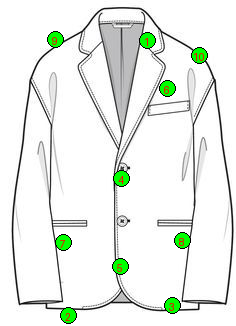
\includegraphics[width=0.35\textwidth,height=12cm,keepaspectratio]{blazer_illustration_front.png}% INSERT IMAGE HERE
};
\end{tikzpicture}
\end{center}
&
% Right side - Attributes Table
\specificationtable{
Component & Specification\\
1 & Collar and lapel region: Construct with firm interfacing for crisp shaping, ensuring precise topstitching.\\
2 & Lower left hem corner: Reinforce with additional stitching to prevent wear and tear.\\
3 & Lower right hem corner: Mirror construction of left side, maintaining symmetrical hemline.\\
4 & Upper button placement: Reinforce behind button for extra stability, aligned with lapel roll.\\
5 & Second button placement: Include backing button or reinforcement to avoid strain on front panel.\\
6 & Chest pocket area: Welt pocket with interfacing, maintain a clean edge with bar-tacked corners.\\
7 & Left front pocket area: Flap pocket with sturdy interfacing, sewn with consistent alignment.\\
8 & Right front pocket area: Symmetrical to left pocket, ensuring even pocket alignment.\\
9 & Left shoulder seam: Slight shoulder pad insertion for structure, smooth transition into the sleeve.\\
10 & Right shoulder seam: Matching shape and fill, balancing armscye for ease of movement.\\
}
\end{tabular}

\vspace{0.5cm}

% MEASUREMENTS TABLE
\measurementtable{
Shoulder Width (cm) & Chest (cm) & Waist (cm) & Sleeve (cm) & Front Length (cm) & Lapel Width (cm) & Pocket (cm) \\
46 & 110 & 102 & 64 & 78 & 8 & 14 \\
}

\newpage

% BACK VIEW SECTION
\techsection{BACK VIEW}
\vspace{-0.3cm}

\begin{tabular}{p{0.49\textwidth}|p{0.49\textwidth}}
% Left side
\begin{center}
\begin{tikzpicture}
\node[draw=bordercolor, line width=1pt, inner sep=4pt, fill=white, rounded corners=2pt] {
    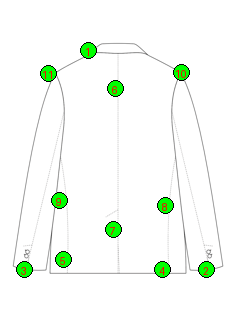
\includegraphics[width=0.35\textwidth,height=12cm,keepaspectratio]{blazer_illustration_back.png}% INSERT IMAGE HERE
};
\end{tikzpicture}
\end{center}
&
% Right side - Attributes Table
\specificationtable{
Component & Specification\\
1 & Upper back neckline: Seam carefully shaped, slightly reinforced for collar support.\\
2 & Right lower hem edge: Triple-stitched for durability, matching front hem height.\\
3 & Left lower hem edge: Mirror finish of right side hem, ensuring uniform bottom line.\\
4 & Right vent start: Reinforced at stress points for ease of movement.\\
5 & Left cuff area: Button closure with small placket, neatly topstitched.\\
6 & Center back seam: Curved for natural drape, reinforced with topstitching.\\
7 & Mid-back waist area: Incorporate slight taper for shaping, maintain balanced fit.\\
8 & Right elbow zone: Sleeve shaped for comfortable bend, lightly interfaced.\\
9 & Left elbow zone: Matching shaping with symmetrical stitching details.\\
10 & Right shoulder area: Contoured to match front shoulder seam for consistent armhole fit.\\
11 & Left shoulder area: Mirroring right side for even shoulder slope and comfort.\\
}
\end{tabular}

\vspace{0.5cm}

% MEASUREMENTS TABLE
\measurementtable{
Across Shoulders (cm) & Back Width (cm) & Waist (cm) & Center Back Length (cm) & Sleeve (cm) & Vent Length (cm) & Hem Width (cm) \\
48 & 42 & 102 & 79 & 64 & 25 & 55 \\
}

\newpage

% REFERENCE IMAGES SECTION
\techsection{REFERENCE}
\vspace{-0.3cm}

\begin{tabular}{p{0.49\textwidth}|p{0.49\textwidth}}
% Left side - Place reference images here
\begin{center}
\begin{tikzpicture}
\node[draw=bordercolor, line width=1pt, inner sep=4pt, fill=white, rounded corners=2pt] {
    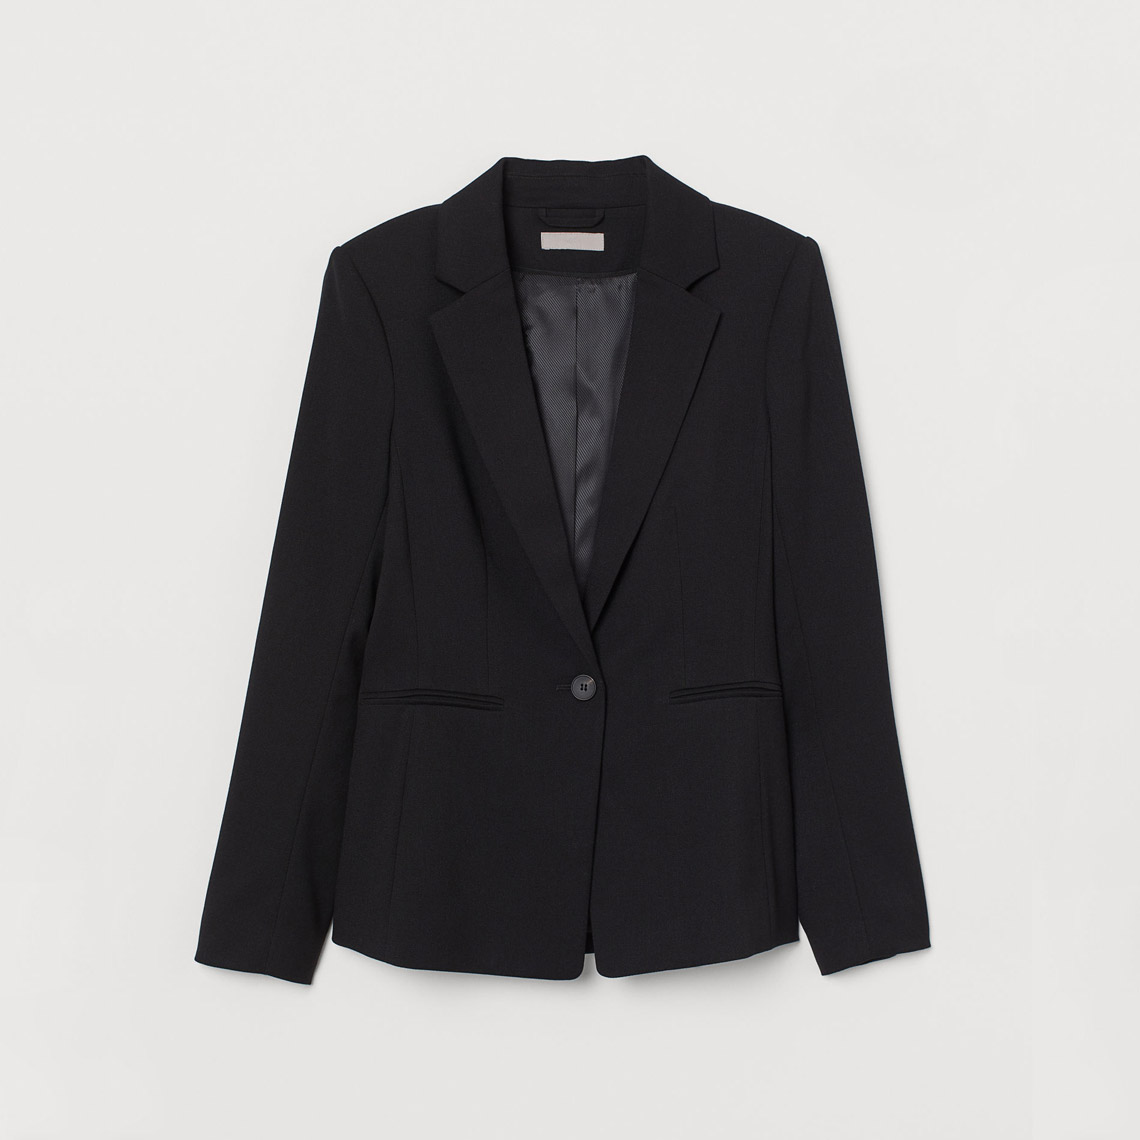
\includegraphics[width=0.35\textwidth,height=12cm,keepaspectratio]{reference_blazer.png}
};
\end{tikzpicture}
\end{center}
&
% Right side - Description of reference image
\begin{center}
\begin{tabular}{|p{10cm}|}
\hline
\rowcolor{mediumblue}\multicolumn{1}{|c|}{\textcolor{white}{\textbf{Description}}} \\
\hline
\large A black single-button blazer with a structured silhouette, notched lapel, and minimal pockets. It provides a sleek and versatile foundation for the design.
\\
\hline
\end{tabular}
\end{center}
\end{tabular}

\newpage

% BILL OF MATERIALS
\techsection{BILL OF MATERIALS}
\vspace{-0.3cm}
\noindent\begin{tabularx}{\textwidth}{|>{\columncolor{lightblue}\bfseries}X|X|>{\raggedleft\arraybackslash}X|}
\hline
\rowcolor{mediumblue}\textcolor{white}{\textbf{Material}} & \textcolor{white}{\textbf{Description}} & \textcolor{white}{\textbf{Estimated Price}} \\
\hline
Main Fabric & Wool-poly blend & \$15/yard \\
\hline
Lining & Polyester Lining, 100 gsm & \$8/yard \\
\hline
Buttons & Black plastic or horn & \$2 per set \\
\hline
Interfacing & Fusible Interfacing & \$1/yard \\
\hline
\end{tabularx}

\vspace{0.7cm}

\newpage

% CARE INSTRUCTIONS
\techsection{CARE INSTRUCTIONS}
\vspace{-0.3cm}

\noindent\begin{tabularx}{\textwidth}{|X|}
\hline
\begin{minipage}[t]{\linewidth}
\vspace{0.3cm}
\large
\begin{itemize}
  \item Dry clean recommended.
  \item Do not bleach.
  \item Do not tumble dry.
  \item Iron on low heat if necessary.
\end{itemize}
\vspace{0.3cm}
\end{minipage} \\
\hline
\end{tabularx}

\vspace{0.7cm}

\newpage

% ADDITIONAL COMMENTS
\techsection{ADDITIONAL COMMENTS}
\vspace{-0.3cm}
\noindent\begin{tabularx}{\textwidth}{|X|}
\hline
\large Please have this done by next week. \\
\hline
\end{tabularx}

\end{document}